\documentclass[12pt,a4paper,twocolumn]{article}
\usepackage[latin1]{inputenc}
\usepackage{amsmath}
\usepackage{amsthm}
\usepackage{amsfonts}
\usepackage{amssymb}
\usepackage{graphicx}
\usepackage{cite}
\usepackage{tikz}
\usetikzlibrary{arrows,shapes,automata,petri,shadows}
\usepackage[left=2cm,right=2cm,top=2cm,bottom=2cm]{geometry}

\newtheorem{myDef}{Definition}

\author{Josiah Hanna, David Tamez, and Xiaorong Zhu}
\title{Evolving Petri Networks for High Level Robot Control}
\begin{document}



\maketitle

\begin{abstract}

Petri networks are mathematical models for representing processes. One application of Petri networks is modelling high level robot control. In previous work, this has involved hand coding the Petri networks using the designers knowledge of the target domain. In this paper we show how to use an evolutionary algorithm to automatically generate a correct Petri network for a specific task. 

\end{abstract}

\section{Introduction}

\section{Background}

\subsection{Petri Networks}
Petri networks are mathematical models for representing processes. Formally we define Petri nets as:
\begin{myDef}
A Petri Net is defined as a tuple $(P,T,F,M,W)$ where $P$ is a set of place nodes, $T$ is a set of transition nodes, $F$ is a set of arcs in either $P \times T$ or $T \times P$, $M: P \rightarrow Z$ is an initial marking, and $W: F \rightarrow Z$ is an arc weight function.
\end{myDef}
\begin{figure}[h]
\centering
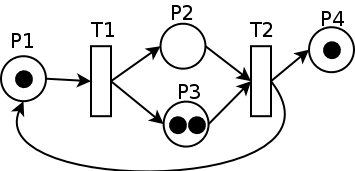
\includegraphics[scale=0.25]{petri_net.png}
\caption[]{An example Petri network \label{exampleNet}}
\end{figure}
Petri nets have many applications including data analysis, simulation of systems, and showing correctness of a system. The techniques we present are for the application of high level robot control. The disadvantage of Petri nets for this application is that they must be hand coded using designer knowledge of the domain. For complex tasks this is not very scalable.

\subsection{The NEAT Algorithm}

The Neuroevolution of Augmenting Topologies (NEAT) algorithm is a powerful tool for evolving the structure and weights of an artificial neural network. NEAT specifies the structure of a neural network with node and connection genes. Each gene has an innovation number associated with it which allows genomes of networks with very different structures to match up during cross over operations. Mutation operations can change the structure of a new network by addings nodes or connections between nodes. In addition to the normal evolutionary algorithm techniques, NEAT utilizes speciation give new topological innovations time to develop \cite{neat}. Finally, NEAT starts with a uniform population of simple networks thus biasing the search towards simpler networks.

\section{Related Work}



\section{Evolution of Petri Networks}

We propose that the Neuroevolution of Augmenting Topologies (NEAT) could be used to evolve Petri Nets. Like neural networks, Petri nets are a combination of nodes and connections with weights on the connections. We only must modify the genome specification and the mutation operators to adapt NEAT to evolve Petri nets. With these changes NEAT becomes the PetriNEAT algorithm. The following subsections describe these changes in more detail.

\subsection{Petri Net Genes}

PetriNEAT evolves individuals that are specified by a genome. A genome contains genes of two types: nodes and arcs. Node genes can represent either places or transitions depending on a specified type. The type of node determines what other node properties will be expressed. For instance, transition nodes do not express the initial tokens trait. Alternatively, transitions and place nodes can be viewed as having their own type of gene however it was simpler to only implicitly do this. All gene values are integers with the exception of Action I.D.s which are bit strings. This allows us to mutate actions easier.

\begin{figure}
%\begin{table}
\centering
\begin{tabular}{|c|}
\hline
Node Gene\\ \hline
I.D. \\
Type \\
Initial Tokens \\
Action I.D. \\
Condition \\
\hline
\end{tabular}
\begin{tabular}{|c|}
\hline
Arc Gene\\ \hline
Place I.D.\\
Transition I.D.\\
Weight \\
 - \\
 -\\
\hline
\end{tabular}
%\end{table}
\caption{PetriNEAT uses two types of genes: node and arc genes.}
\end{figure}


\subsection{Petri Net Mutation Operators}

PetriNEAT uses very similar mutation operators to the original NEAT algorithm. The only change is that each mutation must result in a valid network. Our operators are:
\begin{itemize}
\item \emph{Mutate{\_}Add{\_}Node:} Increases the number of transitions or places in the network
\item \emph{Mutate{\_}Add{\_}Link:}  Increases connectivity of the network
\item \emph{Mutate{\_}Node:}  Changes the token count for place nodes. Changes the action associated with transitions.
\item \emph{Mutate{\_}Link:} Changes the weight of the link.
\end{itemize}

Mutations are applied when reproducing the top individuals of each species. The Mutate Add Link operator adds a link between a random place and transition node when an offspring is created. This mutation occurs with probability 0.1. Mutating initial token counts and link weights is done by either incrementing or decrementing with equal probabilities. These mutations occur with probability 0.1. For transition nodes, a mutation can flip bits in the action I.D. with probability 0.5. 

  \begin{figure}
    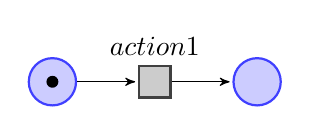
\begin{tikzpicture}[node distance=1.3cm,>=stealth',bend angle=45,auto]
  \tikzstyle{place}=[circle,thick,draw=blue!75,fill=blue!20,minimum size=6mm]
  \tikzstyle{transition}=[rectangle,thick,draw=black!75,
              fill=black!20,minimum size=4mm]
    \node [place,tokens=1,xshift=5cm] (p1){};
    \node [transition] (t1) [right of=p1, label=above:$action1$] {}  edge [pre] (p1);
    \node [place] (p2)  [right of=t1] {} edge [pre] (t1);
\end{tikzpicture}
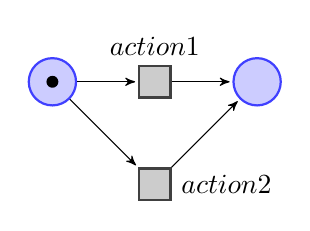
\begin{tikzpicture}[node distance=1.3cm,>=stealth',bend angle=45,auto]
  \tikzstyle{place}=[circle,thick,draw=blue!75,fill=blue!20,minimum size=6mm]
  \tikzstyle{transition}=[rectangle,thick,draw=black!75,
        fill=black!20,minimum size=4mm]
    \node [place,tokens=1] (p1){};
    \node [transition] (t1) [right of=p1, label=above:$action1$] {}  edge [pre] (p1);
    \node [place] (p2)  [right of=t1] {} edge [pre] (t1);
    \node [transition] (p3) [below of=t1, label=right:$action2$] {} edge [pre] (p1) edge [post] (p2);
\end{tikzpicture}

\caption{Adding connectivity}
\end{figure}

\begin{figure}
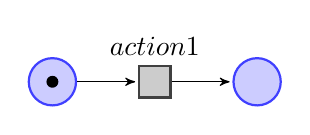
\begin{tikzpicture}[node distance=1.3cm,>=stealth',bend angle=45,auto]
  \tikzstyle{place}=[circle,thick,draw=blue!75,fill=blue!20,minimum size=6mm]
  \tikzstyle{transition}=[rectangle,thick,draw=black!75,
              fill=black!20,minimum size=4mm]
    \node [place,tokens=1, yshift=5em] (p1){};
    \node [transition] (t1) [right of=p1, label=above:$action1$] {}  edge [pre] (p1);
    \node [place] (p2)  [right of=t1] {} edge [pre] (t1);
\end{tikzpicture}
\hspace{5mm}
 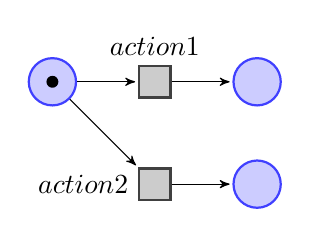
\begin{tikzpicture}[node distance=1.3cm,>=stealth',bend angle=45,auto]
  \tikzstyle{place}=[circle,thick,draw=blue!75,fill=blue!20,minimum size=6mm]
  \tikzstyle{transition}=[rectangle,thick,draw=black!75,
        fill=black!20,minimum size=4mm]
    \node [place,tokens=1] (p1){};
    \node [transition] (t1) [right of=p1, label=above:$action1$] {}  edge [pre] (p1);
    \node [place] (p2)  [right of=t1] {} edge [pre] (t1);
	\node [place] (p4) [below of=p2] {};    
    \node [transition] (p3) [below of=t1, label=left:$action2$] {} edge [pre] (p1) edge [post] (p4);
    
\end{tikzpicture}
\caption{Grow the network}
\end{figure}



\section{Experiments}

\begin{figure}[h]

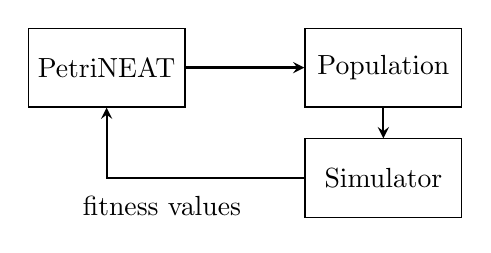
\begin{tikzpicture}

\tikzstyle{line} = [draw, -stealth, thick]
\tikzstyle{elli}=[draw, ellipse, minimum height=8mm, text width=5em, text centered]
\tikzstyle{block} = [draw, rectangle,  text width=5em, text centered, minimum height=10mm, node distance=10em]

\node [block] (population) {Population};
\node [block, below of=population, yshift=6em] (simulator) {Simulator};
\node [block, left of=population] (algorithm) {PetriNEAT};

%arrows
\path [line] (algorithm) -- (population);
\path [line] (population) -- (simulator);
\path [line] (simulator) -| node[yshift=0.5em, xshift=2em, yshift=-1.5em] {fitness values} (algorithm);
\end{tikzpicture}
\caption{Each individual is produced by the PetriNEAT algorithm and then evaluated in the simulator. The fitness values are then used to guide PetriNEAT in producing the next generation of the population.}
\end{figure}

We evolve Petri net solutions for a robot moving towards a goal in a grid world.
\begin{figure}
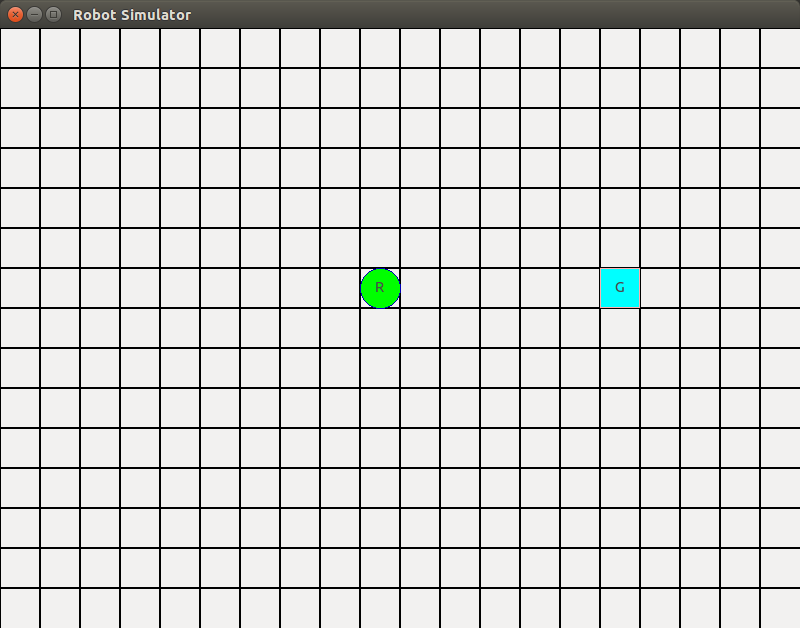
\includegraphics[trim = 80mm 80mm 20mm 70mm, clip, width = 2.4in, height = 1.6in]{robot_sim.png}
\end{figure}
We define the fitness of a potential solution to be:
$$fitness = \frac{2^{goalReached}}{1.0 + finalDistanceFromGoal + actionsTaken}$$

\subsection{Experimental Set Up}

\subsection{Results}


  \begin{figure}
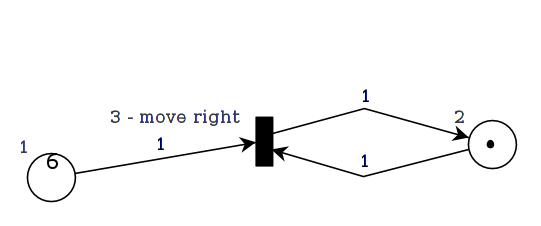
\includegraphics[scale=0.3]{PetriNet_1_1}

\end{figure}
\vspace{-5ex}
\begin{figure}
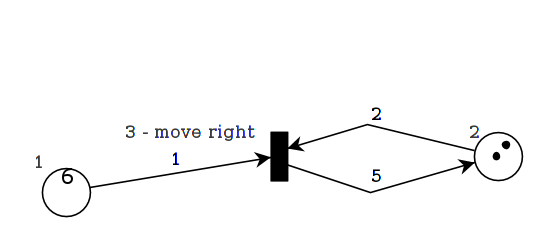
\includegraphics[scale=0.3,width=2in]{PetriNet_1_2}

\end{figure}
  \begin{figure}
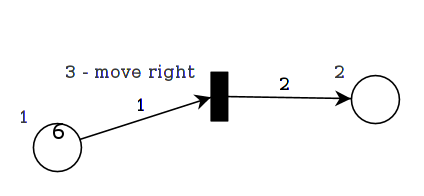
\includegraphics[scale=0.3]{PetriNet_1_3}
\vspace{-5ex}
\end{figure}
 \begin{figure}
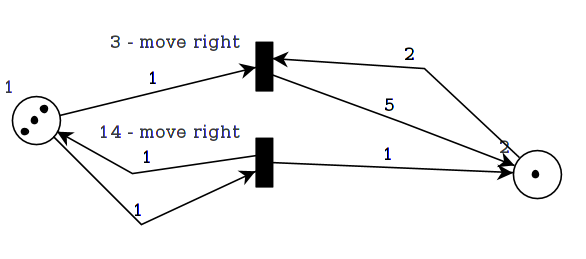
\includegraphics[scale=0.3, width=2in]{PetriNet_1_4}

\end{figure}

\begin{figure}
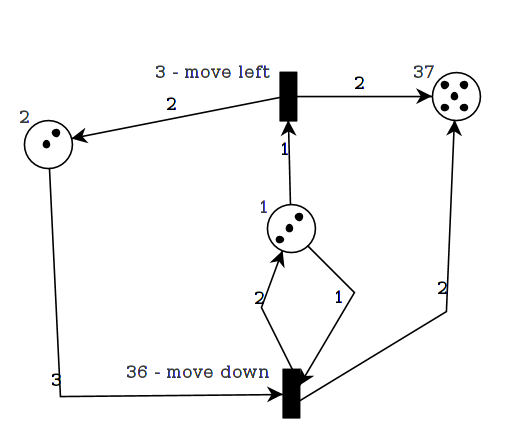
\includegraphics[scale=0.3]{PetriNet_2_1}
\end{figure}

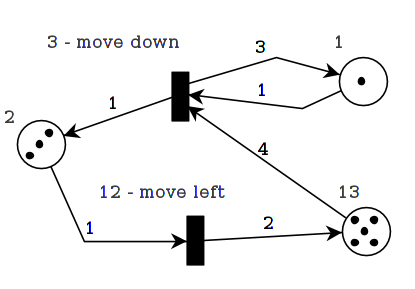
\includegraphics[scale=0.3]{PetriNet_2_2}

\section{Discussion and Future Work}

Conclusion: It is possible to evolve Petri nets
\begin{itemize}
\item Petri net weights, markings, and structure can adapt to improve network fitness.
\item Networks evolved through mutation can solve a given task.
\item Simple building blocks can create compound actions.
\end{itemize}

The next steps in exploring Petri net evolution are:
\begin{enumerate}
\item Add cross over operations to the evolutionary algorithm.
\item Explore different mutation operators.
\item Generate more complex types of Petri networks.
\item Increase the complexity of our target task.
\item Add methods to combine Petri nets into hierarchies.
\item Use reachability graph to simplify network.
\end{enumerate}

\section{Conclusion}

\bibliographystyle{plain}
\bibliography{project}

\end{document}